
Baseado nesses resultados, podemos propor a seguinte heurística para identificar comunidades com maior probabilidade de serem câmaras de eco:

\begin{itemize}
	\item 1. Calcular os valores para todas as métricas para cada comunidade.
	\item 2. Ponderar cada métrica pelo peso correspondente ao PCA.
	\item 3. Ordenar as comunidades com base nos valores ponderados.
\end{itemize}

Comunidades com valores altos nesta classificação terão maior probabilidade de ser câmaras de eco. Isso ocorre porque, conforme indicado pelo PCA, estas comunidades teriam alta densidade, alta força de câmara de eco e baixa exposição média, todos fatores que contribuem para a formação de câmaras de eco.

Concluindo, ao incorporar os insights do PCA com as métricas fornecidas, podemos desenvolver uma abordagem mais informada e precisa para identificar câmaras de eco em redes sociais. Esta heurística pode ser usada como uma ferramenta valiosa para moderadores e administradores de redes sociais, permitindo-lhes identificar e abordar proativamente comunidades que têm propensão a se tornarem câmaras de eco.

Essa abordagem ilustra a importância de combinar medidas globais e locais na detecção de câmaras de eco. Enquanto medidas globais como o GEC fornecem uma visão geral da tendência da rede para formar câmaras de eco, medidas locais são necessárias para identificar câmaras de eco específicas e entender a dinâmica dentro dessas comunidades. A classe EchoChamberDetector fornece uma implementação computacional do nosso teorema de probabilidade de câmaras de eco, permitindo a identificação de potenciais câmaras de eco em redes sociais. No entanto, é importante notar que a detecção de câmaras de eco é um problema complexo que pode não ser totalmente capturado por qualquer conjunto de heurísticas. Portanto, é sempre uma boa ideia testar essas heurísticas em uma variedade de dados e contextos para ver como elas se comportam. Nesse contexto, a análise de componentes principais nos ajudou a entender melhor quais métricas são mais importantes para a formação de câmaras de eco e como elas podem ser usadas para identificar comunidades com maior probabilidade de serem câmaras de eco.

\subsection{Derivando parâmetros beta}

Na implementação da classe EchoChamberDetector, a escolha dos valores dos parâmetros beta é um aspecto crucial para a eficácia do modelo. Esses parâmetros, que quantificam a influência de várias estatísticas descritivas na probabilidade de formação de câmaras de eco, podem ser derivados de várias maneiras, dependendo do contexto específico e das características da rede. No caso da rede social Colab, os valores dos parâmetros beta podem ser informados pelas estatísticas da rede, conforme apresentado na \autoref{tab:colab_gephi_statistics}.

O parâmetro $\beta_1$, que representa a densidade da comunidade, pode ser informado pelo coeficiente de agrupamento médio da rede. Uma rede com um coeficiente de agrupamento médio alto tende a ter comunidades densas. O parâmetro $\beta_2$, que representa a homogeneidade das opiniões, pode ser informado pelo número de comunidades na rede. Uma rede com muitas comunidades tende a ter opiniões mais homogêneas dentro de cada comunidade. O parâmetro $\beta_3$, que representa as conexões externas, pode ser informado pelo número de componentes fracamente conectados na rede. Uma rede com muitos componentes fracamente conectados tende a ter menos conexões externas. O parâmetro $\beta_4$, que representa o efeito dos influenciadores, pode ser informado pela mudança da soma da centralidade de eigenvector na rede. Uma rede com uma alta mudança da soma da centralidade de eigenvector tende a ter influenciadores mais influentes. O parâmetro $\beta_5$, que representa a exposição média, pode ser informado pelo comprimento médio do caminho na rede. Uma rede com um comprimento médio de caminho longo tende a ter uma exposição média mais alta. Finalmente, o parâmetro $\beta_6$, que representa o GEC, pode ser informado pela modularidade da rede. Uma rede com alta modularidade tende a ter um GEC mais alto.

Os valores betas derivados desse racional podem ser aplicados a rede do Colab como um todo, mas precisam ser adaptados para diferentes topologias de rede. Por exemplo o valor para numero de comunidades e o valor para numero de componentes fracamente conectados mudam drasticamente ao comprar cidades como Caruarú, Recife e Niterói, por exemplo. Dessa forma, incorporamos o cálculo desses racionais na implementação da classe EchoChamberDetector através do método estático, \texttt{derive\_betas}, que calcula esses valores iniciais com base nas estatísticas da rede dado um grafo G. Isso permite uma abordagem mais informada e adaptativa para a detecção de câmaras de eco, que pode ser ajustada para diferentes redes e contextos. Para testar a classe, criamos um modelo aleatório que gera um grafo de rede social com pelo menos uma câmara de eco.

\section{Simulações de Câmaras de Eco com Modelos Aleatórios}

A análise de redes sociais é um campo que se beneficia significativamente da aplicação de modelos estatísticos, e um dos mais influentes é o modelo Markoviano. Nomeado em homenagem ao matemático russo Andrey Markov, este modelo tem sido uma ferramenta fundamental em várias disciplinas desde o início do século XX. A característica definidora de um modelo Markoviano é a sua propriedade de "sem memória", onde a probabilidade de transição para um estado futuro depende exclusivamente do estado presente, independentemente de como o sistema chegou ao seu estado atual.

Esta propriedade de "sem memória" simplifica a análise e a computação de sistemas complexos, tornando os modelos Markovianos uma escolha atraente para uma variedade de aplicações. No entanto, a aplicação dos modelos Markovianos na análise de redes sociais é particularmente interessante. Neste contexto, os nós da rede representam indivíduos ou entidades, e as arestas representam relações ou interações entre eles. Os modelos Markovianos podem ser usados para modelar a evolução dessas redes ao longo do tempo, levando em conta a dependência entre as interações.

Uma extensão desses modelos, conhecida como Modelos Exponenciais de Grafos Aleatórios (ERGMs), permite a modelagem de dependências mais complexas entre as arestas, capturando assim a estrutura de interação global da rede. Estes modelos representam uma abordagem inovadora para a análise de redes sociais, oferecendo vantagens significativas em relação aos métodos tradicionais de análise de grafos. Enquanto as técnicas tradicionais tendem a se concentrar em propriedades individuais dos nós ou arestas, os ERGMs permitem a modelagem de dependências complexas entre as arestas, capturando assim a estrutura de interação global da rede.

Os ERGMs são particularmente úteis para modelar fenômenos sociais complexos, como a formação de câmaras de eco. A análise das redes da Colab, até o presente momento, tem sido conduzida utilizando técnicas convencionais de análise de redes, tais como medidas de centralidade e modularidade, aplicadas a capturas estáticas da rede. Essas capturas representam o estado da rede em pontos específicos no tempo, fornecendo uma visão instantânea das conexões entre os usuários. O modelo de dados disponibilizado pelo Colab, apresentado em detalhes na \autoref{sec:colab_data_analysis}, consiste em uma lista de arestas que representam as conexões entre os usuários, juntamente com informações temporais que indicam quando essas conexões foram estabelecidas e possivelmente removidas. Além disso, cada usuário é caracterizado por uma série de atributos, como descrito na \autoref{tab:user_model}. A estrutura desses dados, que capturam tanto a topologia da rede quanto as características dos usuários, torna a análise baseada em ERGMs particularmente apropriada, pois permite a modelagem de dependências complexas entre as arestas, proporcionando uma representação mais precisa da estrutura de interação global da rede.

Nesse contexto, os Modelos Exponenciais de Grafos Aleatórios (ERGMs), uma extensão dos modelos Markovianos, oferecem uma abordagem metodológica robusta. Os ERGMs permitem a modelagem de dependências complexas entre as arestas, proporcionando uma representação mais precisa da estrutura de interação global da rede, mesmo em uma visão estática. Esta capacidade é particularmente relevante para a detecção de câmaras de eco, fenômenos caracterizados por comunidades altamente interconectadas dentro de uma rede, onde a informação circula predominantemente dentro do grupo. A literatura recente fornece vários exemplos de como os ERGMs podem ser usados para modelar a formação de câmaras de eco. Por exemplo, \citeonline{2022_Sun} usaram o ERGM para calcular o efeito da câmara de eco e o efeito de três mecanismos de interação na câmara de eco. Eles descobriram que o comportamento de imitação e interação entre grupos está positivamente relacionado ao efeito da câmara de eco.

\subsection{Modelando a rede social Colab com ERGMs}

O propósito de utilizar simulações ERGM neste estudo é alcançar a capacidade de criar redes sociais sintéticas que se assemelhem à rede Colab afim de testar e otimizar as heurísticas de detecção de câmaras de eco. Para atingir esse objetivo, implementamos um modelo ERGM para descrever a rede social Colab, permitindo assim a identificação e o estudo detalhado das câmaras de eco presentes nessa rede.  O modelo é especificado usando a notação formulaica do pacote ERGM, onde a fórmula define as estatísticas descritivas que descrevem a estrutura da rede e as preferências dos usuários. A seguir apresentamos a fórmula do modelo ERGM proposto para a rede social Colab:

Seja $G = (V, E)$ o grafo da rede social, onde $V$ é o conjunto de nós (usuários) e $E$ é o conjunto de arestas (conexões). Queremos modelar a probabilidade de ocorrência desse grafo com base em diferentes características e atributos dos nós e das arestas. A equação do modelo é definida como:

\[
	P(G) = \frac{e^{\sum_i \beta_i s_i(G)}}{C(\boldsymbol{\beta})}
\]

em que $P(G)$ é a probabilidade de ocorrência do grafo $G$, $\beta_i$ são os parâmetros do modelo, $s_i(G)$ são as estatísticas do modelo e $C(\boldsymbol{\beta})$ é uma constante de normalização.

As estatísticas do modelo capturam diferentes aspectos da rede social e são representadas por $s_i(G)$. Neste modelo específico, as estatísticas incluem:

\begin{itemize}
	\item $s_{\text{edges}}(G)$: O número de arestas presentes no grafo $G$. Essa estatística captura a formação de conexões entre os usuários.

	\item $s_{\text{nodematch("location")}}(G)$: O número de pares de nós que compartilham a mesma localização. Essa estatística reflete a tendência dos usuários em seguir outros usuários da mesma cidade.

	\item $s_{\text{istar(1)}}(G)$: O número de estrelas com um nó central em cada nó. Essa estatística modela a formação de conexões em torno de um usuário central.

	\item $s_{\text{ostar(1)}}(G)$: O número de estrelas com um nó central apontando para cada nó. Essa estatística captura a formação de conexões direcionadas para um usuário central.

	\item $s_{\text{nodematch("age")}}(G)$: O número de pares de nós que compartilham a mesma faixa etária. Essa estatística reflete a preferência dos usuários em seguir outros usuários da mesma idade.

	\item $s_{\text{gwidegree}}(G)$: A distribuição dos graus de entrada ponderados dos nós na rede. Essa estatística modela a propagação de popularidade entre os usuários.

	\item $s_{\text{gwodegree}}(G)$: A distribuição dos graus de saída ponderados dos nós na rede. Essa estatística captura a propagação de atividade entre os usuários.

	\item $s_{\text{nodefactor("age")}}(G)$: A distribuição dos fatores dos nós relacionados à idade. Essa estatística reflete a preferência dos usuários com base na idade.

	\item $s_{\text{gwdsp}}(G)$: A distribuição das distâncias geodésicas entre os nós na rede. Essa estatística considera a proximidade entre os usuários na formação de conexões.

	\item $s_{\text{mutual}}(G)$: O número de conexões mútuas presentes no grafo $G$. Essa estatística captura a existência de conexões bidirecionais entre os usuários.
\end{itemize}

O modelo proposto busca capturar características específicas do Colab e sua dinâmica de rede social colaborativa.

A inclusão da estatística "edges" (arestas) no modelo reflete a importância das conexões entre os usuários. No Colab, os usuários interagem uns com os outros por meio de conexões, seguindo e sendo seguidos. Essas conexões representam o fluxo de informações e colaboração na plataforma. Portanto, é essencial considerar o número de arestas presentes no grafo para modelar a formação dessas conexões.

A estatística "nodematch("location")" (correspondência de nós por localização) foi incluída para capturar a tendência dos usuários em seguir outros usuários da mesma cidade. No Colab, os usuários tendem a se conectar e colaborar com pessoas que estão geograficamente próximas a eles. Isso ocorre porque a colaboração local pode facilitar encontros pessoais, discussões presenciais e o desenvolvimento de projetos conjuntos. Portanto, ao considerar a localização como um fator de correspondência entre os nós, o modelo leva em conta essa preferência dos usuários por conexões locais.

As estatísticas "istar(1)" e "ostar(1)" foram adicionadas para modelar a formação de conexões em torno de um usuário central e a existência de conexões direcionadas para um usuário central, respectivamente. No contexto do Colab, certos usuários podem desempenhar um papel central na rede, sendo altamente conectados e influentes. Esses usuários centrais são frequentemente seguidos por outros usuários e podem ser fontes de informações, ideias e colaborações. Portanto, é relevante considerar a presença de conexões centradas em nós e conexões direcionadas para nós centrais no modelo.

A inclusão da estatística "nodematch("age")" (correspondência de nós por idade) se baseia na observação de que os usuários do Colab podem ter preferências em seguir outros usuários da mesma faixa etária. Isso pode ocorrer devido a interesses comuns, experiências compartilhadas ou abordagens semelhantes para a colaboração. Ao considerar a idade como um fator de correspondência entre os nós, o modelo leva em conta essa preferência dos usuários por conexões com pessoas da mesma faixa etária.

As estatísticas "gwidegree" e "gwodegree" foram incluídas para modelar a propagação de popularidade e atividade na rede do Colab, respectivamente. No contexto da plataforma, certos usuários podem ser mais populares e ativos do que outros. A popularidade pode ser medida pelo número de seguidores de um usuário, enquanto a atividade pode ser quantificada pelo número de pessoas que um usuário segue. Essas estatísticas capturam a disseminação da popularidade e da atividade entre os usuários, refletindo a dinâmica de influência e engajamento social no Colab.

A estatística "nodefactor("age")" foi adicionada para capturar a distribuição dos fatores relacionados à idade dos usuários. No Colab, a idade pode ser um fator importante que influencia as preferências e comportamentos dos usuários. Ao considerar os fatores relacionados à idade dos usuários como uma variável categórica, o modelo pode levar em conta possíveis diferenças nas interações e padrões de conexão com base na idade dos usuários.

Por fim, a estatística "gwdsp" (distância geodésica ponderada) foi incluída para modelar a influência do caminho geodésico na formação de conexões no Colab que representa a menor distância entre dois nós na rede. Ao considerar a distância geodésica ponderada, o modelo pode capturar o efeito da proximidade e acessibilidade na formação de conexões. Isso é relevante, pois usuários mais próximos podem estar mais propensos a interagir e colaborar uns com os outros.

Ao combinar todas essas estatísticas em um único modelo, buscamos capturar as características específicas da rede social colaborativa do Colab. Essas escolhas foram baseadas em observações e conhecimentos prévios sobre a dinâmica da plataforma, levando em consideração a importância das conexões, localização, usuários centrais, preferências relacionadas à idade, popularidade, atividade, fatores categóricos e distâncias geodésicas. O modelo visa fornecer uma representação adequada e abrangente da rede do Colab, permitindo análises mais detalhadas sobre sua estrutura e dinâmica.

\subsubsection*{Implementação de ERGM utilizando a linguagem \textit{R}}

Criamos um conjunto de algoritmos em R descrevevendo a implementaçao do modelo ERGM criado a partir de um sub-sampling do modelo de dados original do Colab contendo 10.000 vértices. Esse grafo original foi utilizado para simulação de grafos de rede com a intenção de converger em um grafo com estrutura similar ao grafo original. O treinamento do modelo funciona por meio de iterações. Cada iteração é uma etapa em que o modelo atualiza os parâmetros com base nos dados observados da rede e compara com as redes simuladas. O objetivo é encontrar um conjunto de parâmetros que melhor explique a estrutura da rede observada.

No início do processo, definimos a fórmula do modelo, que especifica quais características da rede estamos considerando e como elas influenciam a probabilidade dessas características ocorrerem. Durante as iterações, o modelo avalia quão bem a rede observada se ajusta às redes simuladas com base na fórmula do modelo. Ele ajusta os parâmetros para melhorar a correspondência entre a rede observada e as redes simuladas. O processo continua até que o modelo atinja a convergência, ou seja, os parâmetros alcancem um estado estável em que iterações adicionais não resultem em mudanças significativas nos valores dos parâmetros. Ao final das iterações, obtemos as estimativas finais dos parâmetros, que refletem a influência de cada termo na fórmula do modelo na probabilidade de ocorrerem determinadas características na rede. Essas estimativas nos fornecem insights sobre os processos subjacentes que moldam a estrutura da rede, como a formação de conexões entre os usuários com base na localização ou a preferência por seguir outros usuários da mesma faixa etária.

Após desenvolver o modelo baseado em ERGM, realizamos uma série de experimentos para avaliar sua adequação e desempenho. Primeiro, executamos o modelo em nossa rede social colaborativa do Colab, usando o conjunto de dados completo com 10.000 vértices. Em seguida, executamos o modelo em uma série de redes simuladas, geradas a partir do conjunto de dados original. Por fim, comparamos os resultados do modelo com os dados observados e as redes simuladas, avaliando a adequação do modelo e a qualidade de ajuste. A Figura \ref{fig:ergm_diagnostics} mostra os resultados do diagnóstico do modelo, que inclui a comparação entre os dados observados e as redes simuladas, bem como a distribuição dos parâmetros estimados. A comparação entre os dados observados e as redes simuladas mostra que o modelo se ajusta bem aos dados, pois a rede observada está dentro do intervalo de confiança de 85\% das redes simuladas. Além disso, a distribuição dos parâmetros estimados mostra que todos os parâmetros são significativos, pois seus valores estão fora do intervalo de confiança dos parâmetros simulados. Esses resultados indicam que o modelo é adequado para representar a estrutura da rede social do Colab.


\begin{figure}[!htb]
	\caption{Diagnóstico do modelo ERGM}
	\label{fig:ergm_diagnostics}
	\centering
	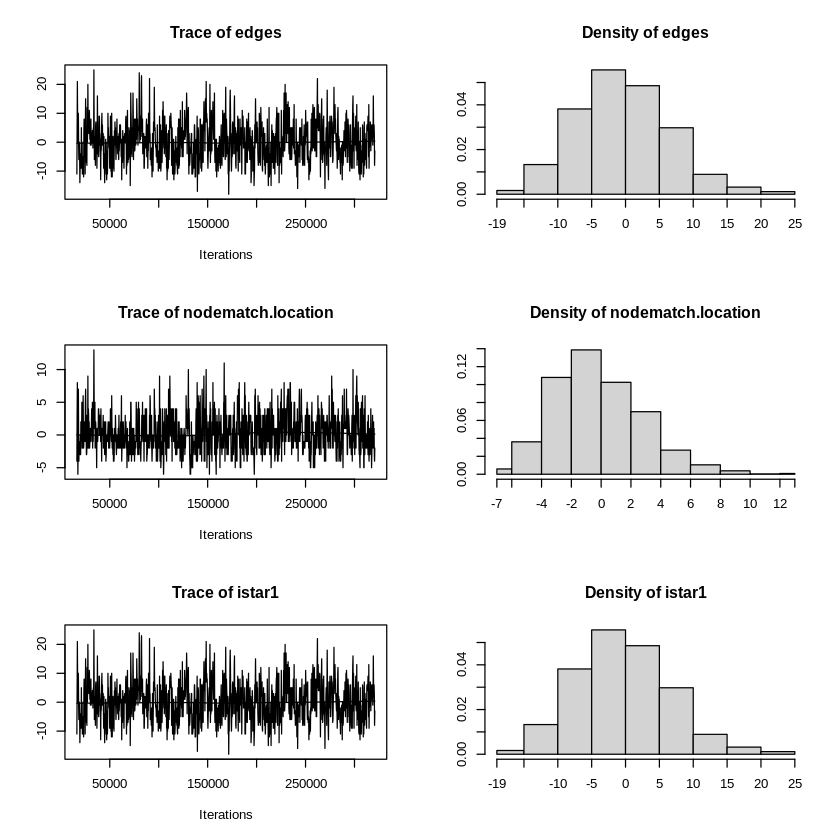
\includegraphics[scale=0.5]{images/ergm_diagnostics.png}
	\fautor
\end{figure}

Após a convergência do modelo, adotamos uma abordagem baseada em simulação para avaliar a capacidade do modelo ERGM em gerar redes que mimetizassem a estrutura da rede social do Colab. Usando o código em R, geramos vários "edgelists" de redes aleatórias. Estas redes simuladas não apenas representaram conexões entre usuários, mas também incorporaram eventos aleatórios, como "likes", comentários e votos em diferentes tipos de eventos relacionados de zeladoria pública. Essa simulação foi essencial para entender o comportamento dinâmico dos usuários na plataforma. Por exemplo, é comum em redes sociais que usuários interajam mais frequentemente com postagens que são relevantes para suas próprias crenças ou interesses em sua proximidade geografica. Ao introduzir eventos aleatórios, buscamos replicar esse comportamento com o objetivo de que as redes simuladas se assemelhassem, tanto quanto possível, à rede real do Colab.

\subsection{Visualizando Câmaras de Eco}

De volta ao Python, podemos utilizar a classe \textttt{NetworkPlotter} para exibir a rede com os nós colorizados baseado nas comunidades identificadas. 

\begin{figure}[!htb]
	\caption{Plot de um rede aleatória gerada pelo modelo ERGM baseado na topologia da rede do Colab}
	\label{fig:ergm_random_network}
	\centering
	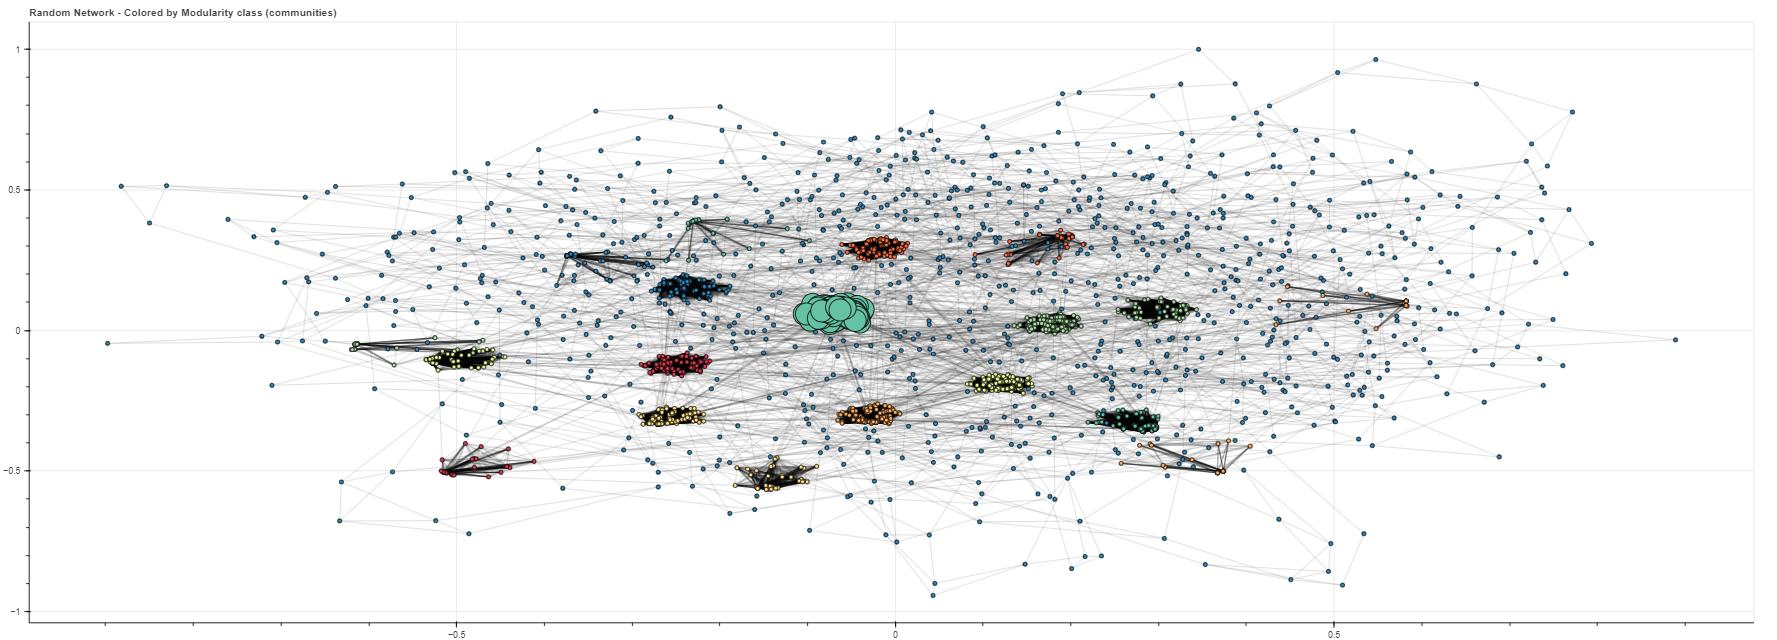
\includegraphics[scale=0.5]{images/ergm_random_network.png}
	\fautor
\end{figure}

\begin{figure}[!htb]
	\caption{Plot da rede ERGM com câmaras de eco identificadas}
	\label{fig:ergm_random_network_echo_chambers}
	\centering
	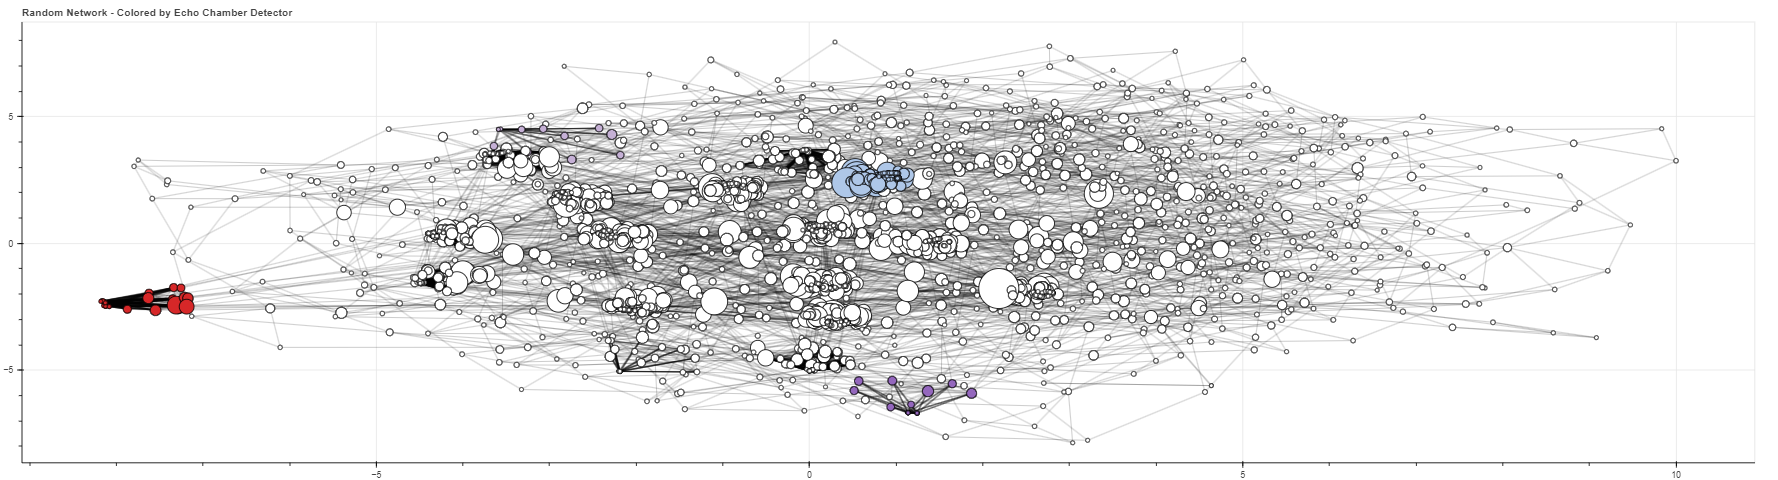
\includegraphics[scale=0.5]{images/ergm_random_network_echo_chambers.png}
	\fautor
\end{figure}
